\documentclass[10pt]{beamer}

% Beamer style
%\usetheme[secheader]{Madrid}
% \usetheme{CambridgeUS}
\useoutertheme{infolines}
\usecolortheme[rgb={0.65,0.15,0.25}]{structure}
% \usefonttheme[onlymath]{serif}
\beamertemplatenavigationsymbolsempty
%\AtBeginSubsection

% Packages
%\usepackage[french]{babel}
\usepackage[latin1]{inputenc}
\usepackage{color}
\usepackage{xspace}
\usepackage{dsfont, stmaryrd}
\usepackage{amsmath, amsfonts, amssymb}
\usepackage{epsfig}
\usepackage{tikz}
\usepackage{url}
\usepackage{/home/robin/LATEX/Biblio/astats}
%\usepackage[all]{xy}
\usepackage{graphicx}

% Commands
% TikZ
\newcommand{\nodesize}{2em}
\newcommand{\edgeunit}{2*\nodesize}
\tikzstyle{hidden}=[draw, circle, fill=gray!50, minimum width=\nodesize, inner sep=0]
\tikzstyle{observed}=[draw, circle, fill=white,minimum width=\nodesize, inner sep=0]
\tikzstyle{eliminated}=[draw, circle, minimum width=\nodesize, color=gray!50, inner sep=0]
\tikzstyle{empty}=[]
\tikzstyle{arrow}=[->, >=latex, line width=1pt]
\tikzstyle{edge}=[-, line width=1pt]
\tikzstyle{dashededge}=[-, dashed, line width=1pt]
\tikzstyle{dashedarrow}=[->, >=latex, dashed, line width=1pt]
\tikzstyle{lightarrow}=[->, >=latex, line width=1pt, fill=gray!50, color=gray!50]

% % TikZ
% \newcommand{\nodesize}{1.8em}
% \newcommand{\edgeunit}{2.2*\nodesize}
% \tikzstyle{hidden}=[draw, circle, fill=gray!50, minimum width=\nodesize, inner sep=0]
% \tikzstyle{observed}=[draw, circle, minimum width=\nodesize, inner sep=0]
% \tikzstyle{eliminated}=[draw, circle, minimum width=\nodesize, color=gray!50, inner sep=0]
% \tikzstyle{empty}=[]
% \tikzstyle{arrow}=[->, >=latex, line width=1pt]
% \tikzstyle{edge}=[-, line width=1pt]
% \tikzstyle{dashedarrow}=[->, >=latex, dashed, line width=1pt]
% \tikzstyle{lightarrow}=[->, >=latex, line width=1pt, fill=gray!50, color=gray!50]


\definecolor{darkred}{rgb}{0.65,0.15,0.25}
\newcommand{\emphase}[1]{\textcolor{darkred}{#1}}
% \newcommand{\emphase}[1]{{#1}}
\newcommand{\paragraph}[1]{\textcolor{darkred}{#1}}
\newcommand{\refer}[1]{{{\textcolor{gray}{{[\cite{#1}]}}}}}
\newcommand{\Refer}[1]{{{\textcolor{gray}{{[#1]}}}}}
\renewcommand{\newblock}{}

% Symbols
\newcommand{\Abf}{{\bf A}}
\newcommand{\Beta}{\text{B}}
\newcommand{\Bcal}{\mathcal{B}}
\newcommand{\BIC}{\text{BIC}}
\newcommand{\Ccal}{\mathcal{C}}
\newcommand{\dd}{\text{~d}}
\newcommand{\dbf}{{\bf d}}
\newcommand{\Dcal}{\mathcal{D}}
\newcommand{\Esp}{\mathbb{E}}
\newcommand{\Ebf}{{\bf E}}
\newcommand{\Ecal}{\mathcal{E}}
\newcommand{\Gcal}{\mathcal{G}}
\newcommand{\Gam}{\mathcal{G}\text{am}}
\newcommand{\Hcal}{\mathcal{H}}
\newcommand{\Ibb}{\mathbb{I}}
\newcommand{\Ibf}{{\bf I}}
\newcommand{\ICL}{\text{ICL}}
\newcommand{\Cov}{\mathbb{C}\text{ov}}
\newcommand{\Corr}{\mathbb{C}\text{orr}}
\newcommand{\Var}{\mathbb{V}}
\newcommand{\Vsf}{\mathsf{V}}
\newcommand{\pen}{\text{pen}}
\newcommand{\Fcal}{\mathcal{F}}
\newcommand{\Hbf}{{\bf H}}
\newcommand{\Jcal}{\mathcal{J}}
\newcommand{\Kbf}{{\bf K}}
\newcommand{\Lcal}{\mathcal{L}}
\newcommand{\Mcal}{\mathcal{M}}
\newcommand{\mbf}{{\bf m}}
\newcommand{\mum}{\mu(\mbf)}
\newcommand{\Ncal}{\mathcal{N}}
\newcommand{\Nbf}{{\bf N}}
\newcommand{\Nm}{N(\mbf)}
\newcommand{\Ocal}{\mathcal{O}}
\newcommand{\Obf}{{\bf 0}}
\newcommand{\Omegas}{\underset{s}{\Omega}}
\newcommand{\Pbf}{{\bf P}}
\newcommand{\Pt}{\widetilde{P}}
\newcommand{\Pcal}{\mathcal{P}}
\newcommand{\Qcal}{\mathcal{Q}}
\newcommand{\Rbb}{\mathbb{R}}
\newcommand{\Rcal}{\mathcal{R}}
\newcommand{\Scal}{\mathcal{S}}
\newcommand{\Tcal}{\mathcal{T}}
\newcommand{\Ucal}{\mathcal{U}}
\newcommand{\Vcal}{\mathcal{V}}
\newcommand{\BP}{\text{BP}}
\newcommand{\EM}{\text{EM}}
\newcommand{\VEM}{\text{VEM}}
\newcommand{\VBEM}{\text{VBEM}}
\newcommand{\cst}{\text{cst}}
\newcommand{\obs}{\text{obs}}
\newcommand{\ra}{\emphase{\mathversion{bold}{$\rightarrow$}~}}
%\newcommand{\transp}{\text{{\tiny $\top$}}}
\newcommand{\transp}{\text{{\tiny \mathversion{bold}{$\top$}}}}
\newcommand{\logit}{\text{logit}\xspace}

% Directory
\newcommand{\fignet}{../../../RESEAUX/EXPOSES/FIGURES}
\newcommand{\figchp}{../../../RUPTURES/EXPOSES/FIGURES}
\newcommand{\figexp}{../../../EXPRESSION/EXPOSES/FIGURES}


%====================================================================
%====================================================================

%====================================================================
%====================================================================
\begin{document}
%====================================================================
%====================================================================

%====================================================================
\title{Some statistical topics in genomics}

\author{S. Robin}

\institute[INRA / AgroParisTech]{INRA / AgroParisTech \\
  \vspace{-.1\textwidth}
  \begin{tabular}{ccccc}
    
\includegraphics[height=.3\textheight]{\fignet/LogoINRA-Couleur} & 
    \hspace{.02\textheight} &
    
\includegraphics[height=.08\textheight]{\fignet/logagroptechsolo} & 
    \hspace{.02\textheight} &
    
\includegraphics[height=.09\textheight]{\fignet/logo-ssb}
    \\ 
  \end{tabular} \\
  \bigskip
  }

\date{July 2016, Berkeley}

%====================================================================
%====================================================================
\maketitle
%====================================================================

%====================================================================
\frame{\frametitle{Topics}
  \tableofcontents
}

%====================================================================
%====================================================================
\section{Differential analysis}
%====================================================================
\frame{\frametitle{Differential analysis}

  \begin{tabular}{cc}
    \begin{tabular}{p{.45\textwidth}}
	 \paragraph{Aim:} Compare conditions $A$ and $B$. \\~
	 
	 Negative binomial model
	 $$
	 Y_{gcr} \sim \Ncal\Bcal(\mu_{gc}, \phi_{?})
	 $$ 
	 
	 Mixture model for over-dispersion:
	 \begin{eqnarray*}
	   Z_g & = & k: \text{disp. group of gene $g$} \\
	   U_{gcr} & \sim & \Gam(\alpha_k, \alpha_k) \\
	   Y_{gcr} & \sim & \Pcal(\mu_{gc} \times U_{gcr}) \\
	 \end{eqnarray*}
	 
	 \bigskip
	 \ra \paragraph{Single cell?}
    \end{tabular}
    & 
    \hspace{-.075\textwidth}
    \begin{tabular}{p{.5\textwidth}}
	 \includegraphics[width=.45\textwidth]{\figexp/BPR15-Biometrics-Fig1b} \\
	 \includegraphics[width=.4\textwidth]{\figexp/BPR15-Biometrics-Fig2b} \\
	 \refer{BPR15} 
    \end{tabular}
  \end{tabular}

}

%====================================================================
%====================================================================
\section{Change-point detection}
%====================================================================
\frame{\frametitle{Change-point detection: Genome-wide}

  \begin{tabular}{cc}
    \begin{tabular}{p{.45\textwidth}}
    \paragraph{Aim:} Find changes in a signal along the genome \\
    - Copy number variations \\
    - Gene detection
    
    \bigskip
    \paragraph{Algorithmic Issues:} \\
    - Pruned dynamic programming \refer{CKL14} \\
    - Model selection (how many breaks?) \refer{ClL14}
    
    \bigskip
    \paragraph{Extension to HiC data} \refer{LDM14} \\
    - Works by V. Brault
    \end{tabular}
    & 
    \hspace{-.05\textwidth}
    \begin{tabular}{p{.5\textwidth}}
    	 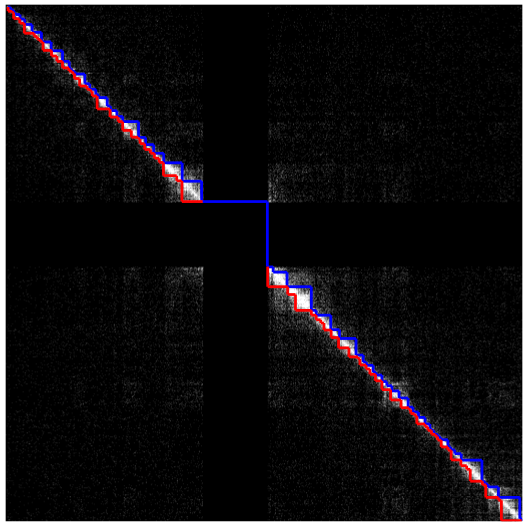
\includegraphics[width=.45\textwidth]{\figchp/LDM14-Fig7b} 
    \end{tabular}
  \end{tabular}
}

%====================================================================
\frame{\frametitle{Change-point detection: Local analysis}

  \begin{tabular}{cc}
    \begin{tabular}{p{.45\textwidth}}
    \paragraph{Precisely locate changes} \\
    - Exact Bayesian inference \\
    - Exact credibility intervals \refer{RLR11}
    
    \bigskip
    \paragraph{Compare break locations} \\
    - Posterior distribution of the shift \\
    - Posterior prob. of no shift \\
    - Alternative splicing in yeast? 
    \refer{ClR14}
    \end{tabular}
    & 
    \hspace{-.075\textwidth}
    \begin{tabular}{p{.5\textwidth}}
	 \includegraphics[width=.45\textwidth]{\figchp/ClR14-Fig4.pdf} \\
	 \includegraphics[width=.45\textwidth, height=.4\textheight]{\figchp/ClR14-Fig5.pdf} 
    \end{tabular}
  \end{tabular}

}

%====================================================================
%====================================================================
\section{Metagenomics}
%====================================================================
\frame{\frametitle{Metagenomics: Latent block-model}

  \begin{tabular}{cc}
    \begin{tabular}{p{.45\textwidth}}
	 \paragraph{Data:} $Y_{ijr} =$ 'abundance' of species $i$ in site $j$ (rep. $r$). \\
	 ~\\
	 
	 \paragraph{Aim:} find preferential relations between species and sites. \\
	 ~\\
	 
	 \paragraph{Latent block model:}
	 \begin{eqnarray*}
	 Z_i & = & k: \text{group of species $i$} \\
	 W_j & = & \ell: \text{group of site $i$} \\
	 Y_{ij} & \sim & \Ncal\Bcal(a_i b_{jr} \emphase{\alpha_{k\ell}}, \phi_?) \\
	 \end{eqnarray*}
	 $a_i =$ mean abundance of species $i$, \\
	 $b_{jr} =$ sequencing depth in sample $jr$.
	 

    \end{tabular}
    & 
    \hspace{-.05\textwidth}
    \begin{tabular}{p{.5\textwidth}}
    Variational EM inference. \\
    ~\\
    \includegraphics[width=.5\textwidth]{\fignet/Aub14-JDS-Table.pdf} 
    \end{tabular}
  \end{tabular}
}

%====================================================================
\frame{\frametitle{Metagenomics: Multivariate analysis}

	 \paragraph{'HydroGene' project:} Characterization of metagenomic sample from Tara-Ocean. \\
	 ~\\
	 
	 \paragraph{Observations:} Frequency of $k$-mers in each sample, with $k = 10, 20, 30$. \\
	 ~\\
	 
	 Need for basic tools for sample comparison, multivariate analysis, dimension reduction, $k$-mer selection \\
	 - that are dedicated to count data and \\
	 - that scale to deal with $4^{30} \simeq 10^{18}$ $k$-mers.
 }

%====================================================================
%====================================================================
\section{Networks}
%====================================================================
\frame{\frametitle{Network models}

  \begin{tabular}{cc}
    \begin{tabular}{p{.45\textwidth}}
	 \emphase{Observed} network with $n$ entities 
	 \\
	 - model its topology \\
	 - classify nodes with similar role 
	 
	 \bigskip
	 Statistics \\
	 - Variational inference \\
	 - Covariates \\
	 - Goodness-of-fit

	 \bigskip
	 Application \\
	 - Social sciences \\
	 - Ecology
	 
	 \bigskip
	 \refer{DPR08} \refer{MRV10} \refer{LaR15}

    \end{tabular}
    & 
    \hspace{-.075\textwidth} 
    \begin{tabular}{p{.5\textwidth}}
    Operon network of {\sl E. coli} \\
	\includegraphics[width=.45\textwidth]{\fignet/im_EcoliVEM}
    \end{tabular}
  \end{tabular}
}

%====================================================================
\frame{\frametitle{Network inference}

  \begin{tabular}{cc}
    \begin{tabular}{p{.45\textwidth}}
	 Observed signal from $n$ entities \\
	 - Try to infer direct links (conditional dependencies) between them \\
	 - e.g. Gaussian graphical models
	 
	 \bigskip
	 Exact Bayesian inference \\
	 - if graph = tree \\
	 - Posterior prob. of each edge \refer{SRS15}
	 
	 \bigskip 
	 Extension \\
	 - Change-points in graphical model \\
	 - Network rewiring \refer{ScR16}
    \end{tabular}
    & 
    \hspace{-.075\textwidth}
    \begin{tabular}{p{.5\textwidth}}
    \includegraphics[width=.45\textwidth]{\fignet/ScR16-Fig1} \\
    ~ \\~ \\
    \includegraphics[width=.45\textwidth]{\fignet/ScR16-Fig8} \\
    \includegraphics[width=.45\textwidth]{\fignet/ScR16-Fig9} 
    \end{tabular}
  \end{tabular}
}

%====================================================================
\frame[allowframebreaks]{ \frametitle{References}
{\tiny
  \bibliography{../../../../Biblio/BibGene}
%   \bibliographystyle{/home/robin/LATEX/Biblio/astats}
  \bibliographystyle{plain}
  }
}


%====================================================================
%====================================================================
\end{document}
%====================================================================
%====================================================================

  \begin{tabular}{cc}
    \begin{tabular}{p{.5\textwidth}}
    \end{tabular}
    & 
    \hspace{-.075\textwidth}
    \begin{tabular}{p{.5\textwidth}}
    \end{tabular}
  \end{tabular}

